% THIS DOCUMENT IS FOLLOWS THE VOLERE TEMPLATE BY Suzanne Robertson and James Robertson
% ONLY THE SECTION HEADINGS ARE PROVIDED
%
% Initial draft from https://github.com/Dieblich/volere
%
% Risks are removed because they are covered by the Hazard Analysis
\documentclass[12pt]{article}

\usepackage{booktabs}
\usepackage{tabularx}
\usepackage{longtable}
\usepackage{hyperref}
\usepackage{cite}
\usepackage{enumitem}
\usepackage{longtable}
\usepackage{array} % Optional: For better column formatting
\usepackage{amssymb}
\usepackage{amsmath}
\usepackage{framed}

\hypersetup{
    bookmarks=true,         % show bookmarks bar?
      colorlinks=true,      % false: boxed links; true: colored links
    linkcolor=red,          % color of internal links (change box color with linkbordercolor)
    citecolor=green,        % color of links to bibliography
    filecolor=magenta,      % color of file links
    urlcolor=cyan           % color of external links
}
\usepackage{graphicx}
\graphicspath{ {./images/} } % relative path

\newcommand{\lips}{\textit{Insert your content here.}}

\input{../Comments}
\input{../Common}

\begin{document}

\title{Software Requirements Specification for \progname: An audio-to-sheet-music generator} 
\author{\authname}
\date{\today}
	
\maketitle
\thispagestyle{empty}

~\newpage

\pagenumbering{roman}

\tableofcontents

~\newpage

\section*{Revision History}

\begin{tabularx}{\textwidth}{p{3cm}p{2cm}X}
\toprule {\textbf{Date}} & {\textbf{Version}} & {\textbf{Notes}}\\
\midrule
11/10/2024 & 0 & Initial Revision\\
30/01/2025 & 0.1 & \href{https://github.com/emilyperica/ScoreGen/issues/96}{Issue \#96}\\
30/01/2025 & 0.2 & \href{https://github.com/emilyperica/ScoreGen/issues/92}{Issue \#92}\\
30/01/2025 & 0.3 & \href{https://github.com/emilyperica/ScoreGen/issues/128}{Issue \#128}\\
03/04/2025 & 1.0 & \href{https://github.com/emilyperica/ScoreGen/issues/309}{Issue \#309}\\
04/04/2025 & 1.0 & \href{https://github.com/emilyperica/ScoreGen/issues/139}{Issue \#139}\\
\bottomrule
\end{tabularx}

~\\

~\newpage

\pagenumbering{arabic}
\section{Purpose of the Project}
\subsection{User Business}
Music theory is challenging and intimidating to learn for beginners, 
however, the act of playing an instrument does not inherently require 
extensive theoretical knowledge. This project aims to bridge the gap 
between deep theoretical understanding and playing instruments. It 
shall aid musicians with limited music theory knowledge by translating 
analog instrument audio into sheet music and other applicable formats 
that users can use to visualize and document their music-making. The 
project also aims to foster ease of collaboration between musical 
artists for efficient communication. 
\subsection{Goals of the Project}
The goal of the project is to develop a fast, accurate sheet music generator 
paired with an intuitive, user-friendly interface that requires minimal effort 
to learn. If successful, it will encourage the proliferation of musical creativity 
among various audiences. This goal lends itself to several metrics, such as 
computational performance compared to existing products or its reach to certain 
demographics. Ultimately, the benefit of the project will be measured by the number 
of original pieces created.
\section{Stakeholders}
\subsection{Client}
The client is the faculty supervisor of this project, Dr. Martin Von Mohrenschildt. With direct research interests in signal processing and a personal interest in how it relates to 
music, he is investing his own time in the development of the product.
\subsection{Customer}
The archetypal customer is a musician of any skill level, with emphasis based on musicians who have little-to-no music theory knowledge. The customer will utilize the application 
to quickly produce sheet music for either original compositions or existing songs. 
\subsection{Other Stakeholders}
\begin{itemize}
  \item \textbf{Software developers:} Provide the technical knowledge and skill to design and build the system.
  \item \textbf{Composers:} As SMEs, provide the music theory knowledge needed to make the system useful for the customer.
  \item \textbf{Users of music-annotating software:} As SMEs, provide opinions on the features they like or dislike about existing music-annotating softwares. This will help inform the developers on which features of the product to prioritize.
  \item \textbf{Music teachers:} Provide similar support to students that may be replaced by usage of this product. They will have a vested interest in ensuring this product does not encourage bad composing habits in users of the product.
  \item \textbf{Music students:} Similar to the Composers, they will provide the music theory knowledge needed to make the system useful for the customer. However, their input will be from the same learning point of view as the expected user, and thus will have a higher degree of influence on the product.
  \item \textbf{IP lawyers:} Will ensure this product follows fair use and does not infringe on copyrights.
  \item \textbf{Dr. Spencer Smith:} As the course instructor, the performance and outcome of this product will be a direct reflection of his role in the capstone course.
\end{itemize}
\subsection{Hands-On Users of the Project}
\subsubsection*{User Category 1: Beginner Musicians}
\textbf{User Role:} Use this product to create sheet music, either as a learning aid or as a quick alternative to learning music notation.\\
\textbf{Subject matter experience*:} Novice - Little experience with music theory, but likely have a moderate knowledge of music in practicality (i.e., playing an instrument or listening to music). \\
\textbf{Technological experience*:} Novice - May or may not have limited experience with other music-annotating softwares. \\
\textbf{User characteristics:} 
\begin{itemize}
  \item Little to no music theory knowledge
  \item Passionate about music
  \item All ages (i.e., both children and adults)
  \item New to playing instruments
  \item Not comfortable with complex software
  \item Eager to learn
  \item Less willing to spend money
\end{itemize}

\subsubsection*{User Category 2: Composers}
\textbf{User Role:} As masters of music notation and composition, this group will use the product as a practice aid or to quickly make note of composition ideas. \\
\textbf{Subject matter experience*:} Master - have spent years learning and practicing music theory and composition. \\
\textbf{Technological experience*:} Journeyman to Master - Have experience with music-annotating software but haven't necessarily used them extensively. \\
\textbf{User characteristics:}
\begin{itemize}
  \item Advanced music theory knowledge
  \item Passionate about music
  \item 25+ years old
  \item Have a hard time learning new technologies
  \item Willing to spend money
\end{itemize}
\noindent
\textit{*User experience level may be rated as one of novice, journeyman, or master.}

\subsection{Personas}
Harold Style is a software engineering student at McMaster University with a deep interest in music, and loves playing the guitar. Despite his lack of a formal music education, 
he has perfect pitch and thus learns songs by listening to them rather than learn how to read sheet music. However, he recently joined a local rock band called The Beetles who 
expect him to contribute during their songwriting sessions. He needs a quick way to produce sheet music for his own compositions, as well as learn to read the scores written by 
his bandmates. As a future software engineer he enjoys learning new technologies that can make his life easier, and he dislikes reading of any sort.

\subsection{Priorities Assigned to Users}
\textbf{Key users:} Beginner musicians \\
\textbf{Secondary users:} Composers

\subsection{User Participation}
Beginner musicians will have a high level of participation in the creation of system requirements. Their feedback will be especially essential during the early to middle development phases to ensure that the system meets their various needs for simplicity, intuitive design/usage, and music theory assistance.
Composers will have a moderate level of participation in the creation of system requiremens, slightly less than that of the Beginner Musician group. Their subject matter expertise will be useful in creating relevant requirements to ensure precision of audio transcription and its overall score editing capabilities.
\subsection{Maintenance Users and Service Technicians}
This product will be maintained by a software development team, consisting of software developers, UI/UX designers, test engineers, and a project manager. 
Users will receive product support directly from the customer support team, and IP lawyers will be engaged as necessary to address matters of intellectual property.

\section{Mandated Constraints}
\subsection{Solution Constraints}
\subsubsection*{Technology Stack}
\textbf{Description}: The app shall be developed using a fast for the core signal processing to handle real-time calculations and a robust, secure, and easy-to-configure language for backend logic.\\
\textbf{Rationale}: Signal processing needs to be done quickly and effieciently to be done in real time, and the backend must be secure while handling user information.\\
\textbf{Fit Criterion}: The final product shall process signals quickly and all sensitive user information is secured and nothing gets exposed.
\subsubsection*{Open-Source Libraries}
\textbf{Description}: The app shall use open-source libraries and frameworks where applicable to save both time and money.\\
\textbf{Rationale}: The use of open-source libraries ensures cost-effectiveness and allows for community-driven improvements and support.\\
\textbf{Fit Criterion}: All third-party libraries used in the project must be licensed under open-source agreements such as MIT, GPL, or Apache licenses which allow for free use.

\subsection{Implementation Environment of the Current System}
\subsubsection*{Hardware Specifications}
\textbf{Description}: The app shall run on personal computers with a minimum of 8GB RAM, a dual-core processor, and 256GB of available storage space, which is the minimum according to general concensus~\cite{music-specs}.\\
\textbf{Rationale}: These hardware specifications are typical of the devices used by musicians and producers, ensuring the app performs efficiently.\\
\textbf{Fit Criterion}: The app must pass performance tests on machines meeting the minimum hardware requirements, with no more than a 5\% reduction in performance under heavy load.
\subsubsection*{Audio Input Devices}
\textbf{Description}: The app shall support standard audio input devices, including USB microphones, and built-in microphones, with audio input via USB, or 3.5mm audio jacks.\\
\textbf{Rationale}: These input devices are commonly used by musicians to capture sound, ensuring the app is compatible with existing hardware setups.\\
\textbf{Fit Criterion}: The app must successfully capture and process audio from these devices, maintaining accurate signal-to-sheet transcription in at least 95\% of test cases.

\subsection{Partner or Collaborative Applications}
\subsubsection*{Music Notation Software}
\textbf{Description}: The app shall collaborate with music notation software that uses MusicXML formats to export sheet music. These can be seen as ‘partner’ applications since they fit very well with a use case for the application.\\
\textbf{Rationale}: Many composers rely on professional notation software to finalize and edit their sheet music, so it’s essential that the app exports accurate, compatible sheet music files.\\
\textbf{Fit Criterion}: The app must support MusicXML files, for version support see section 3.4: Off-the-Shelf Software - Backward Compatability.

\subsection{Off-the-Shelf Software}
\subsubsection*{MusicXML Format for Sheet Music}
\textbf{Description}: The app shall use MusicXML as the primary format for storing and exporting sheet music data.\\
\textbf{Rationale}: MusicXML is the industry-standard format for sheet music interchange between different music notation software, ensuring compatibility with tools like Sibelius, Finale, MuseScore, and other DAWs. Its widespread adoption makes it the best choice for interoperability.\\
\textbf{Fit Criterion}: The app must successfully export sheet music in MusicXML format, ensuring compatibility with the latest versions of major music notation software, without requiring manual adjustments by the user.
\subsubsection*{Backward Compatibility}
\textbf{Description}: The app shall support both current and older versions of the MusicXML format to ensure maximum compatibility with various notation tools.\\
\textbf{Rationale}: As different users may be using different versions of music notation software, supporting older MusicXML formats ensures accessibility and broader usability.\\
\textbf{Fit Criterion}: The app must successfully import and export MusicXML files using both the latest version of MusicXML and at least one earlier version (e.g., MusicXML 2.0).

\subsection{Anticipated Workplace Environment}
\subsubsection*{Indoor and Studio-Based Environments}
\textbf{Description}: The app shall be designed primarily for indoor environments, such as home studios, professional recording studios, classrooms, and offices where musicians and composers typically work.\\
\textbf{Rationale}: Most users will be working in controlled indoor environments where factors like lighting and noise levels will vary. The app must function optimally in these settings without relying on environmental conditions.\\
\textbf{Fit Criterion}: The app must be tested in various indoor settings (studios, offices, classrooms) with different lighting and noise levels to ensure usability and performance are not impacted by normal environmental variations.
\subsubsection*{Noise Considerations}
\textbf{Description}: The app shall operate effectively in environments with moderate background noise, such as music rehearsal rooms or live performance spaces, without relying on audible notifications.\\
\textbf{Rationale}: Musicians often work in noisy environments. The app should rely on visual feedback rather than any sound-based notifications and should retain its signal-processing ability (see requirement OE-EP1).\\
\textbf{Fit Criterion}: The app must be tested in environments with background noise levels approaching a signal to noise ratio (SNR) of 2:1, indicating its effectiveness with moderate background noise.
\subsubsection*{Portable Workspaces}
\textbf{Description}: The app shall be designed to accommodate musicians working in mobile or temporary workspaces, such as cafes or on-the-go setups using laptops.\\
\textbf{Rationale}: Musicians often work on the move or in shared spaces where setting up large equipment is impractical. The app must be optimized for laptops with limited screen space and varying internet connectivity.\\
\textbf{Fit Criterion}: The app must be tested for usability on laptops with screen sizes as small as 13 inches.

\subsection{Schedule Constraints}
Schedule constraints are provided by the capstone course itself, for a detailed schedule refer to the \href{https://github.com/emilyperica/ScoreGen/blob/main/docs/DevelopmentPlan/DevelopmentPlan.pdf}{development plan document, section 8.}
\subsection{Budget Constraints}
A maximum budget for this project of \$750 has been identified by the capstone course professors. This amount will likely be fine for our project but additional spending will be approved on a case-by-case basis.
\subsection{Enterprise Constraints}
Since this project is being completed for the McMaster University Capstone course, we must adhere to all constraints provided by the \href{https://gitlab.cas.mcmaster.ca/courses/capstone/-/blob/main/CourseOutline/Capstone_Outline.pdf}{Course Outline Document.}
\section{Naming Conventions and Terminology}
\subsection{Glossary of All Terms, Including Acronyms, Used by Stakeholders
involved in the Project}

\begin{longtable}{|l|p{12cm}|}
\hline
\textbf{Term} & \textbf{Definition} \\ 
\hline
\endfirsthead

\hline
\textbf{Term} & \textbf{Definition} \\ 
\hline
\endhead

\hline
\endfoot

\hline
\endlastfoot

Accidental & A symbol used to raise or lower the pitch of a note from its natural state, such as a sharp, flat, or natural. \\ 
\hline
Barline & A vertical line on the staff that divides the music into measures or bars. \\ 
\hline
Bar & A segment of time defined by a given number of beats, typically indicated by vertical lines on a staff. \\ 
\hline
Beat & The basic unit of time in music, often associated with a pulse. \\ 
\hline
Chord & A combination of three or more notes played simultaneously. \\ 
\hline
Chord Chart & A visual representation of the chords used in a song, often used by guitarists and other instrumentalists. \\ 
\hline
Clef & A symbol placed at the beginning of the staff that indicates the pitch of the notes on the staff, such as treble clef (G clef) or bass clef (F clef). \\ 
\hline
Common Time & A musical pattern in which there are four crotchets in a bar. \\ 
\hline
DAW & Digital Audio Workstation. \\ 
\hline
Dynamics & How quietly or loudly a piece of music is played. \\ 
\hline
Final Barline & A double barline indicating the end of a piece of music. \\ 
\hline
HCD & Human-Centered Design. \\ 
\hline
Key Signature & In Western musical notation, a key signature is a set of sharp, flat, or rarely, natural symbols placed on the staff at the beginning of a section of music. \\ 
\hline
Major & A musical scale characterized by a specific pattern of whole and half steps, typically producing a bright or happy sound. \\ 
\hline
Minor & A musical scale that differs from the major scale by having a lowered third degree, typically producing a darker or sadder sound. \\ 
\hline
MIDI & Musical Instrument Digital Interface. \\ 
\hline
Monophonic & Using only one line of music, unaccompanied by any other voices or instruments. \\ 
\hline
MP3 & MPEG-1 Audio Layer 3. \\ 
\hline
MusicXML & Standard open format for exchanging digital sheet music. \\ 
\hline
MVP & Minimum Viable Product. \\ 
\hline
Notation & The system of writing music to represent pitches, rhythms, and dynamics. \\ 
\hline
Note & A symbol representing a musical sound, characterized by its pitch and duration. \\ 
\hline
Rest & A symbol indicating a period of silence in a piece of music. \\ 
\hline
PII & Personal Identifiable Information. \\ 
\hline
Polyphonic & The simultaneous combination of two or more tones or melodic lines. \\ 
\hline
Rhythm & The pattern of sounds and silences in music. \\ 
\hline
SNR & Signal to Noise Ratio. \\ 
\hline
Staff & A set of five horizontal lines and four spaces that represent different pitches for musical notation. \\ 
\hline
Time Signature & Definition 3. \\ 
\hline
UI & User Interface. \\ 
\hline
WAV & Waveform Audio File Format. \\ 
\hline

\end{longtable}

\section{Relevant Facts And Assumptions}
\subsection{Relevant Facts}
\begin{itemize}
  \item This project is under irregular time constraints, given that it is 
  for an undergraduate-level software engineering course. 
  \item Digitizing and transcribing polyphonic audio from multiple instruments
   is a difficult task and may be unachievable due to the aforementioned time constraints. 
  \item Many products are currently available as alternatives to what this project hopes 
  to accomplish. The team will use these products and their functionalities as metrics for success.
\end{itemize}
\subsection{Business Rules}
\begin{enumerate}
  \item Instrument Support
  \begin{itemize}
    \item The application only supports a predefined list of instruments.
    \item No instruments may be added by the user to the predefined list.
  \end{itemize}
  \item Music Theory Compliance
  \begin{itemize}
    \item The application must generate score sheets that adhere to basic music 
    theory rules (e.g., correct note placement, no overlapping notes, etc.).
    \item The application must generate a score sheet within a reasonable amount of time
    to ensure a smooth user experience. 
  \end{itemize}
  \item Ownership
  \begin{itemize}
    \item The application must clearly identify and display the creator/owner of the score.
  \end{itemize}
\end{enumerate}
\subsection{Assumptions}
Assumptions are seperated into two categories based on the effect their falsehood will have 
on the application:
\begin{enumerate}
  \item Should the following assumptions be false, the application will be unusable:
  \begin{itemize}
    \item Users of the application have access to the hardware required, such as a music 
    interface or quality microphone.
    \item Users have access to a desktop or portable computer to use the application.
  \end{itemize}
  \item Should the following assumptions be false, the application will perform at sub-optimally: 
  \begin{itemize}
    \item The operational environment has low levels of background noise.
    \item The human voice is not considered an instrument that the application can handle input from.
    \item Users have a superficial level of understanding of music theory in order to understand 
    what the application does.
  \end{itemize}
\end{enumerate}

\section{The Scope of the Work}
\subsection{The Current Situation}
The following activity diagram illustrates the workflow of manual score sheet generation, the process
which the application intends to improve upon.\\\\
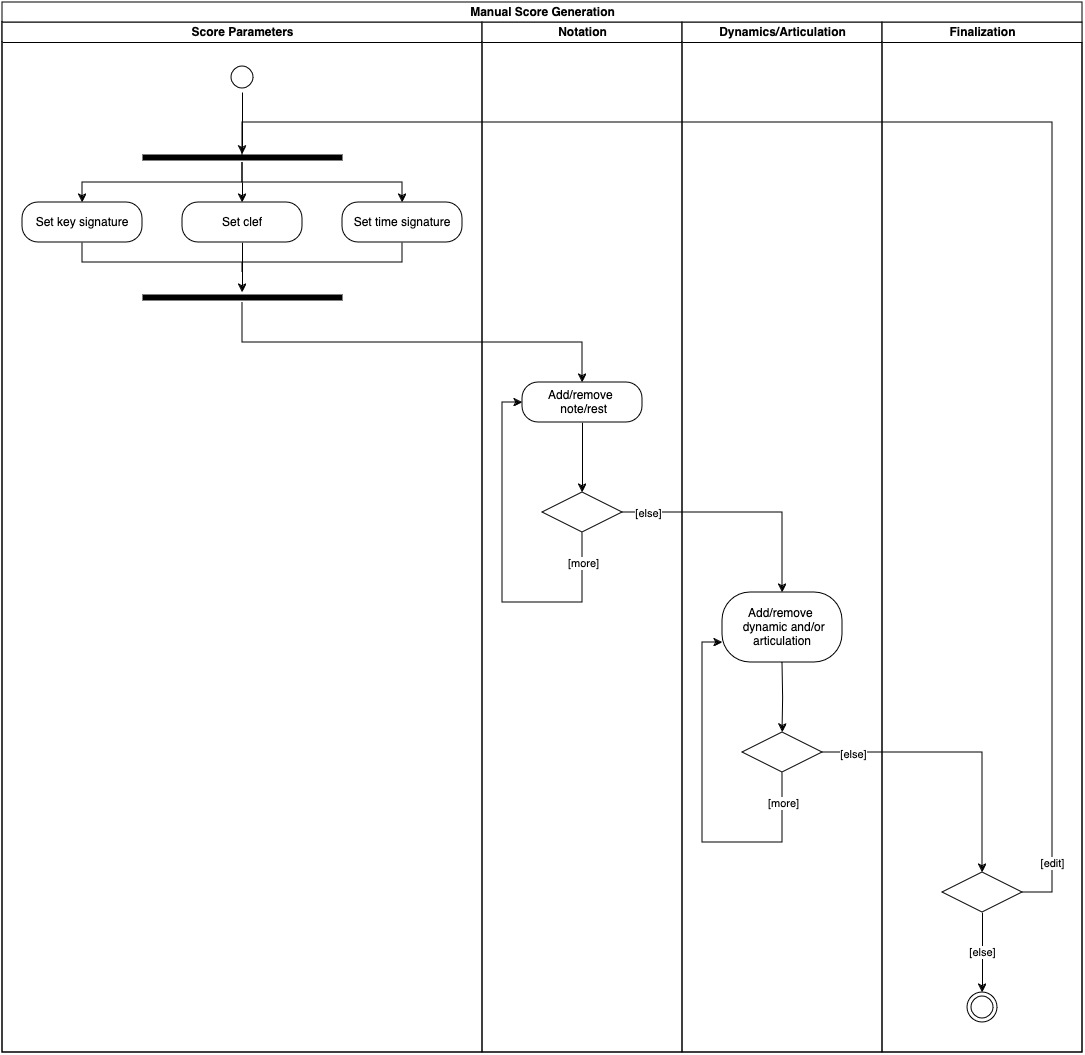
\includegraphics[width=\textwidth]{SRS-manual-score-process-revised.png}
\subsection{The Context of the Work}
The diagram below shows the context in which the development of the application is taking place. It shows
adjacent systems and their associated inputs and outputs as it relates to the application and it's work. \\\\
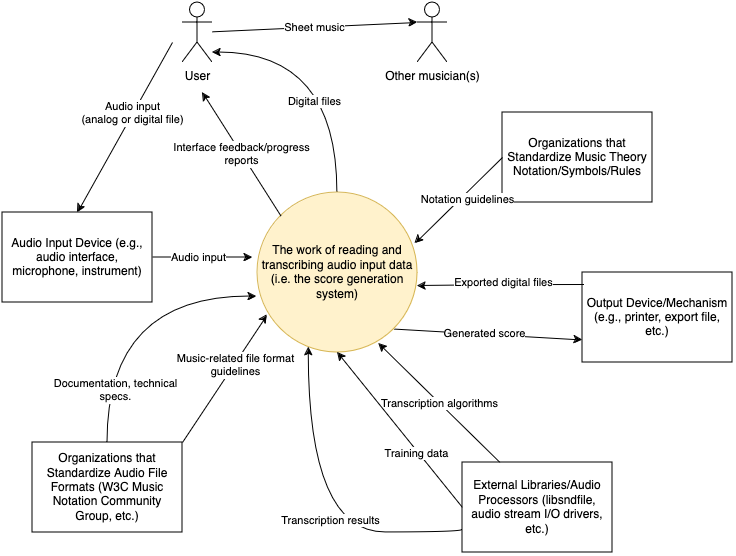
\includegraphics[width=\textwidth]{SRS-contex-diagram-revised.png}

\subsection{Work Partitioning}
The table below summarizes the business events that might be triggered by adjacent organizations
or application users themselves.\\
\begingroup
\renewcommand{\arraystretch}{1.25}
\begin{tabular}{|>{\raggedright}p{3cm}|>{\raggedright}p{4.25cm}|>{\raggedright\arraybackslash}p{6cm}|}
  \hline
  EVENT NAME & INPUT/OUTPUT & SUMMARY OF BUC \\
  \hline
  BE1. User provides audio input. & Audio input (IN) & Process the input audio, digitize if necessary.\\
  \hline
  BE2. Audio transcription. & Transcription results (IN) & Record the notes transcribed. \\
  \hline
  BE3. Score completion. & Generated score (OUT) & Finalize the transcription results into proper music notation/symbols.\\
  \hline
  BE4. Export files. & Exported digital files (IN)  & Convert the generated score into a digital file format for export (see BE6.).\\
  \hline
  BE5. Progress reports. & Interface feedback/progress reports (OUT) & Provide visual indicators to user of transcription status.\\
  \hline
  BE6. Share sheet music. & Digital files (OUT)  & Output the exportable file format (see BE4.).\\
  \hline
\end{tabular}
\endgroup

\subsection{Specifying a Business Use Case (BUC)}
The use case diagram below has been used to specify the details of the BUC 
associated with BE1.\\
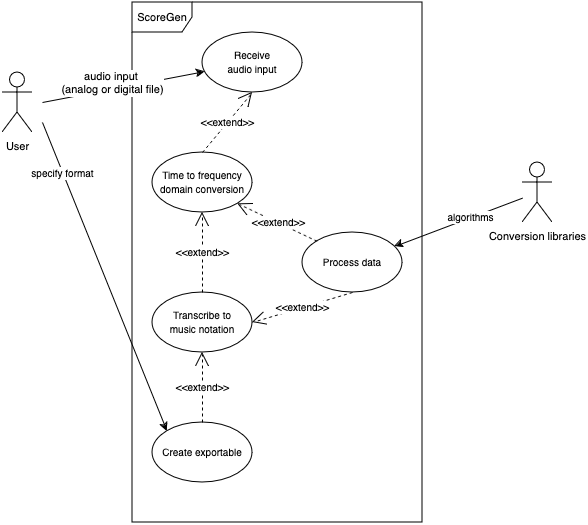
\includegraphics[width=\textwidth]{BUC-revised.png}

\section{Business Data Model and Data Dictionary}
\subsection{Business Data Model}
A first-cut UML class diagram has been used to model the data entities relevant to the scope of the work. This
abstractly describes the relationship between these entities. For definitions and attributes see section \ref{dataDict} Data Dictionary.\\
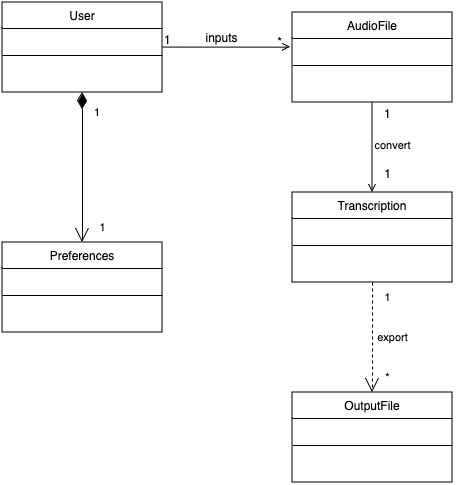
\includegraphics[scale=0.75]{SRS-data-model.png}

\subsection{Data Dictionary} \label{dataDict}
\begingroup
\renewcommand{\arraystretch}{1.25}
\begin{longtable}{|>{\raggedright}p{3cm}|>{\raggedright}p{5.5cm}|>{\raggedright\arraybackslash}p{4cm}|}
  \hline
  NAME & CONTENT & TYPE \\
  \hline
  User & userID + name + preferences & Class\\
  \hline
  Preferences & prefID + userID + instrument + preferredInput & Class \\
  \hline
  AudioFile & audioID + inFileName + format + userID + uploadDate & Class\\
  \hline
  Transcription & transcID + audioID + outputFormat + creationDate + outFileName  & Class \\
  \hline
  OutputFile & outputID + outFileName + fileType  & Class \\
  \hline
  *ID & Unique identifier for distinguishing between entities & Attribute/Element \\
  \hline
  name & Name of the user, for ownership purposes  & Attribute/Element \\
  \hline
  preferences & Data related to user interface preferences  & Attribute/Element \\
  \hline
  instrument & The musical instrument the user has selected to use for input  & Attribute/Element \\
  \hline
  preferredInput & Type of input the user will use (e.g., digital files, analog input)  & Attribute/Element \\
  \hline
  inFileName & Name given to the file that stores input data & Attribute/Element \\
  \hline
  format & The format of the input file (e.g., WAV, MP3, etc.) & Attribute/Element \\
  \hline
  uploadDate & *DD/MM/YYYY*\\ For file management and ownership purposes & Attribute/Element \\
  \hline
  outputFormat & The format that the exportable output file will use & Attribute/Element \\
  \hline
  creationDate & *DD/MM/YYYY*\\For ownership purposes & Attribute/Element \\
  \hline
  outFileName & Name given to the file that stores output data & Attribute/Element \\
  \hline
  fileType & The format that the exportable output file will use & Attribute/Element \\
  \hline
\end{longtable}
\endgroup

\section{The Scope of the Product}
\subsection{Product Boundary}
Input: ScoreGen will be designed to take in and process music data which can be converted to a MIDI or musicXML file representation. The audio should not have excessive noise, or other degradation of quality which could impact the ability to clearly distinguish notes. The input will also be intended to be mono or polyphonic with a singular instrument. The input volume should remain consistent and sufficiently loud, and the user microphone should be correctly calibrated to ensure accuracy by avoiding pitch drift.
\\
Output: The resulting music file will aim to capture the pitch and length of individual notes or chords, but will not capture accents, dynamics, or tempo markings, as well as other advanced elements. If the system detects that a note cannot be reliably transcribed (due to unclear input), it will leave that note blank on the sheet and prompt the user to review the section manually.
\subsection{Product Use Case}
\subsubsection*{UC1: Record and Transcribe}
\textbf{Description:} Musician plays an instrument, and the system transcribes it into sheet music in real-time. \\
\textbf{Actors:} Musician, Desktop App \\
\textbf{Preconditions:} Musician has a working microphone and is playing a supported instrument. \\
\textbf{Basic Flow:}
\begin{enumerate}
    \item Musician plays the instrument.
    \item The system listens through the mic.
    \item Sheet music is generated.
\end{enumerate}
\textbf{Alternate Flow:}
\begin{itemize}
    \item If the note is unclear, the system skips it and warns the user.
\end{itemize}
\textbf{Postconditions:} Sheet music is generated and displayed to the user. 

\subsubsection*{UC2: Edit Transcription}
\textbf{Description:} Musician reviews and edits the generated sheet music if there are missing or incorrect notes. \\
\textbf{Actors:} Musician, Desktop App \\
\textbf{Preconditions:} Sheet music has already been generated from a recording. \\
\textbf{Basic Flow:}
\begin{enumerate}
    \item Musician views the transcription.
    \item Edits or corrects notes as needed.
    \item Saves the updated sheet.
\end{enumerate}
\textbf{Alternate Flow:}
\begin{itemize}
    \item Musician manually inserts missed or unclear notes.
    \item Musician deletes incorrect notes.
\end{itemize}
\textbf{Postconditions:} Musician has an edited, correct version of the sheet music.

\subsubsection*{UC3: Save and Export}
\textbf{Description:} Save the sheet music in a chosen format (e.g., PDF, MIDI, musicXML). \\
\textbf{Actors:} Musician, Desktop App \\
\textbf{Preconditions:} Sheet music is completed and reviewed. \\
\textbf{Basic Flow:}
\begin{enumerate}
    \item Musician chooses the save option.
    \item Selects a file format (PDF, MIDI, musicXML).
    \item System exports the file.
\end{enumerate}
\textbf{Alternate Flow:}
\begin{itemize}
    \item If export fails, the system provides an error message and suggests retrying.
\end{itemize}
\textbf{Postconditions:} The sheet music file is saved in the selected format.

\subsubsection*{UC4: Instrument Setup}
\textbf{Description:} Select instrument type before recording (e.g., piano, guitar). \\
\textbf{Actors:} Musician, Desktop App \\
\textbf{Preconditions:} Desktop app is open, and the user is ready to begin recording. \\
\textbf{Basic Flow:}
\begin{enumerate}
    \item Musician selects the instrument.
    \item System optimizes transcription settings for the chosen instrument.
\end{enumerate}
\textbf{Alternate Flow:}
\begin{itemize}
    \item If no instrument is selected, default settings for piano are used.
\end{itemize}
\textbf{Postconditions:} System is ready to accurately transcribe the chosen instrument.

\subsubsection*{UC5: Error Warning}
\textbf{Description:} System warns if it cannot hear or recognize a note during the recording process. \\
\textbf{Actors:} Musician, Desktop App \\
\textbf{Preconditions:} Musician is actively recording. \\
\textbf{Basic Flow:}
\begin{enumerate}
    \item System detects a missing or unclear note.
    \item A warning is displayed to the user.
\end{enumerate}
\textbf{Alternate Flow:}
\begin{itemize}
    \item The system may suggest trying again or inserting the note manually post-recording.
\end{itemize}
\textbf{Postconditions:} Musician is informed about missing notes and is directed on how to take corrective action, which may involve editing within the app or using a third-party tool depending on available features.

\subsubsection*{UC6: Playback of Transcription}
\textbf{Description:} Musician can play back the recorded notes in the desktop app to review transcription accuracy. \\
\textbf{Actors:} Musician, Desktop App \\
\textbf{Preconditions:} Transcription has been generated from a recording. \\
\textbf{Basic Flow:}
\begin{enumerate}
    \item Musician selects the playback option.
    \item System plays the transcribed notes.
\end{enumerate}
\textbf{Alternate Flow:}
\begin{itemize}
    \item Musician can pause or stop playback to make corrections.
\end{itemize}
\textbf{Postconditions:} Musician reviews the transcription by listening to the played-back notes.


\subsection{Individual Product Use Cases (PUC's)}
\subsubsection*{PUC1: Record Instrument and Transcribe Notes}
\begin{description}[style=nextline]
    \item[Description:] The user records a live performance on an instrument using their microphone, and the system transcribes the notes into sheet music.
    \item[Primary Actor:] Musician
    \item[Trigger:] The user presses the "Record" button.
    \item[Preconditions:]
    \begin{itemize}
        \item User has selected an instrument (e.g., piano, guitar).
        \item User has a working microphone connected to the desktop app.
    \end{itemize}
    \item[Main Success Scenario:]
    \begin{enumerate}
        \item User begins playing the instrument.
        \item System listens to the instrument through the microphone.
        \item Sheet music is displayed on the screen after the user finishes playing.
    \end{enumerate}
    \item[Exceptions:]
    \begin{itemize}
        \item If the system cannot detect a note, it skips the note and warns the user with a notification.
    \end{itemize}
\end{description}

\subsubsection*{PUC2: Save and Export Sheet Music}
\begin{description}[style=nextline]
    \item[Description:] The user saves the transcribed sheet music and exports it in the desired format (PDF, MIDI, musicXML).
    \item[Primary Actor:] Musician
    \item[Trigger:] The user clicks the "Save" or "Export" button.
    \item[Preconditions:]
    \begin{itemize}
        \item The transcription is completed, and the user has reviewed it.
    \end{itemize}
    \item[Main Success Scenario:]
    \begin{enumerate}
        \item The user selects a file format (PDF, MID, musicXMLI).
        \item The system generates a file in the selected format.
        \item The file is saved to the user’s chosen directory.
    \end{enumerate}
    \item[Exceptions:]
    \begin{itemize}
        \item If the export fails due to file system issues, the user is prompted to retry or select another directory.
    \end{itemize}
\end{description}

\subsubsection*{PUC3: Receive Error Warnings for Missing Notes}
\begin{description}[style=nextline]
    \item[Description:] The user is notified if the system cannot detect or accurately transcribe certain notes during recording.
    \item[Primary Actor:] Musician
    \item[Trigger:] The system fails to detect a note.
    \item[Preconditions:]
    \begin{itemize}
        \item User is actively recording their instrument.
    \end{itemize}
    \item[Main Success Scenario:]
    \begin{enumerate}
        \item The system detects a missing note during recording.
        \item A warning message is displayed to the user regarding the missing note.
    \end{enumerate}
    \item[Exceptions:]
    \begin{itemize}
        \item The system suggests the user retry playing the note or to manually insert it later, either within the app or using a third-party tool depending on available features.
    \end{itemize}
\end{description}


\section{Functional Requirements}
\subsection{Audio Input Handling}
\subsubsection*{FR-AI1 Audio Formats} \label{FR-AI1}
\textbf{Requirement:} The system shall accept audio input from users in various formats (e.g., WAV, MP3, AAC). \\
\textbf{Fit Criterion:} The system confirms a succesful upload.
\subsubsection*{FR-AI2 Audio Recording} \label{FR-AI2}
\textbf{Requirement:} The system shall provide a user interface for recording audio directly through a microphone connected to the user's device. \\
\textbf{Fit Criterion:} The system displays a confirmation of reception during real-time recording.
\subsubsection*{FR-AI3 Audio Uploads} \label{FR-AI3}
\textbf{Requirement:} The system shall allow users to upload pre-recorded audio files. \\
\textbf{Fit Criterion:} The system confirms reception of the pre-recorded audio file.
\subsubsection*{FR-AI4 User Input} \label{FR-AI4}
\textbf{Requirement:} The user shall give their instrument (i.e., piano or guitar) to the system as input. \\
\textbf{Fit Criterion:} The interface and concert pitch of the generated sheet music reflect the user's choice.

\subsection{Signal Processing}
\subsubsection*{FR-SP1 Noise Reduction} \label{FR-SP1}
\textbf{Requirement:} The system shall perform noise reduction on the audio input to enhance quality. \\
\textbf{Fit Criterion:} The system generates identical sheet music for input with no background noise and input with a 10\% increase in background noise.
\subsubsection*{FR-SP2 Note Identification} \label{FR-SP2}
\textbf{Requirement:} The system shall analyze the audio to identify pitch and rhythm. \\
\textbf{Fit Criterion:} The generated sheet music visually matches expected notes from a reference audio source and corresponding sheet music.
\subsubsection*{FR-SP3 Key and Time Signature Identification} \label{FR-SP3}
\textbf{Requirement:}	The system shall analyze the audio to identify the key and time signatures. \\
\textbf{Fit Criterion:} The system correctly identifies key and time signatures or their equivalencies (e.g. a minor to C major, common time to cut time) from a reference audio source and corresponding sheet music.
\subsubsection*{FR-SP4 Processing Limitations} \label{FR-SP4}
\textbf{Requirement:} The system gracefully handles overly complex audio input (i.e., it is unable to perform accurate signal processing). \\
\textbf{Fit Criterion:} The system notifies the user that their input cannot be processed.
\subsubsection*{FR-SP5 Polyphonic Audio} \label{FR-SP5}
\textbf{Requirement:} The system shall handle polyphonic audio, allowing for multiple notes to be detected simultaneously. \\
\textbf{Fit Criterion:} The generated sheet music contains chords/simultaneous melody.
\subsubsection*{FR-SP6 Monophonic Audio} \label{FR-SP6}
\textbf{Requirement:} The system shall handle monophonic audio. \\
\textbf{Fit Criterion:} The generated sheet music contains single pitch notes.

\subsection{Sheet Music Generation}
\subsubsection*{FR-SMG1 Notation} \label{FR-SMG1}
\textbf{Requirement:} The system shall generate sheet music in standard music notation based on the parsed audio data. \\
\textbf{Fit Criterion:} The generated sheet music is visually comparable to a reference piece of sheet music.
\subsubsection*{FR-SMG2 Concert Pitch} \label{FR-SMG2}
\textbf{Requirement:} The system shall generate sheet music in the concert pitch of the instrument played in the audio input. \\
\textbf{Fit Criterion:} The generated sheet music visually matches expected notes from a reference audio source and corresponding sheet music.
\subsubsection*{FR-SMG3 Post-Processing Edits} \label{FR-SMG3}
\textbf{Requirement:} The system shall allow users to view and edit the generated sheet music within the application. \\
\textbf{Fit Criterion:} Changes made by the user are reflected in the output files produced during sheet music generation.

\subsection{User Interface}
\subsubsection*{FR-UI1 System Feedback} \label{FR-UI1}
\textbf{Requirement:} The interface shall display processing feedback during audio input. \\
\textbf{Fit Criterion:} Feedback from system is displayed to the user within 2 seconds of their input.
\subsubsection*{FR-UI2 System Documentation} \label{FR-UI2}
\textbf{Requirement:} The system shall provide help documentation and user guides for each feature. \\
\textbf{Fit Criterion:} At least 90\% of users during user testing find the interface easy to navigate.
\subsubsection*{FR-UI3 User Feedback} \label{FR-UI3}
\textbf{Requirement:} The system shall provide a feedback mechanism for users to report issues or suggest features. \\
\textbf{Fit Criterion:} The development team successfully receives user feedback via the feedback mechanism 100\% of the time.
\subsubsection*{FR-UFI4 Customer Support} \label{FR-UI4}
\textbf{Requirement:} The system shall include customer support contact information for troubleshooting. \\
\textbf{Fit Criterion:} At least 90\% of users during user testing report successfull interactions with customer support.

\subsection{Save and Load}
\subsubsection*{FR-SL1 Save} \label{FR-SL1}
\textbf{Requirement:} The system shall allow users to save their work, including both audio files and generated sheet music. \\
\textbf{Fit Criterion:} 100\% of the time when the system reports a succesfull save, the user is succesfully able to locate the audio files and generated sheet music.
\subsubsection*{FR-SL2 Load} \label{FR-SL2}
\textbf{Requirement:} The system shall support loading previously saved audio files and generated sheet music for further editing. \\
\textbf{Fit Criterion:} The system sucesfully retains user progress such that the user may return to their unfinished work seamlessly.


\section{Look and Feel Requirements}
\subsection{Appearance Requirements}
\subsubsection*{LF-A1 Discoverability} \label{LF-A1}
\textbf{Requirement:} Main functionalities of the application interface must have elements that are easily identifiable.\\
\textbf{Fit Criterion:} Upon viewing the product for the first time, 75\% of potential 
users shall be able to locate the interactive element that initiates the score generation process.
\subsubsection*{LF-A2 Colour Cohesion} \label{LF-A2}
\textbf{Requirement:} The application interface must use a consistent color scheme for uniformity.\\
\textbf{Fit Criterion:} The product shall have color guidelines that specify at least three colors to define a palette 
(i.e. primary, secondary, and accent colors).
\subsubsection*{LF-A3 Resolution} \label{LF-A3}
\textbf{Requirement:} The application must use high definition graphics.\\
\textbf{Fit Criterion:} The application will only display images that are of a resolution of 720p or higher.
\subsection{Style Requirements}
\subsubsection*{LF-S1 Authority and Trust} \label{LF-S1}
\textbf{Requirement:} The application must appear authoritative and trustworthy, users are more likely to engage
and remain loyal to an application that is percieved as reliable.\\
\textbf{Fit Criterion:} After one encounter with the application, 70\% of users will agree 
that they can trust the application and how it handles input data.


\section{Usability and Humanity Requirements}
\subsection{Ease of Use Requirements}
\subsubsection*{UH-EOU1 Human Centered Design (HCD)}  \label{UH-EOU1}
\textbf{Requirement:} The app interface must adhere to human-centered design principles to be simple and intuitive to use.\\
\textbf{Fit Criterion:} The user interface must incorporate all four fundamental HCD principles.
\subsection{Personalization and Internationalization Requirements}
\subsubsection*{UH-PI1 Language} \label{UH-PI1}
\textbf{Requirement:} The application must provide support for Canadian English (en-CA).\\
\textbf{Fit Criterion:} All text, labels, and instructions within the application 
shall be presented in Canadian English, with no grammatical or spelling errors.
\subsection{Learning Requirements}
\subsubsection*{UH-L1 Music Theory Familiarity} \label{UH-L1}
\textbf{Requirement:} The application must be usable by users without a formal music theory background. \\
\textbf{Fit Criterion:} After having 10 minutes to familiarize themselves with the app, 95\% of users without a 
formal background will be able to generate a score sheet.
\subsection{Understandability and Politeness Requirements}
\subsubsection*{UH-UP1 Icon Identification} \label{UH-UP1}
\textbf{Requirement:} The app must use symbols and icons that are naturally understandable and/or self-explanatory.\\
\textbf{Fit Criterion:} Users shall be able to easily identify the function of at least 70\% of interactive elements
that have unlabeled icons.
\subsubsection*{UH-UP2 Information Hiding} \label{UH-UP2}
\textbf{Requirement:} The app must hide audio processing and transcription details from the user.\\
\textbf{Fit Criterion:} No user-accessible components of the interface or application shall reveal
implementation-specific or algorithmic solutions used.
\subsection{Accessibility Requirements}
\subsubsection*{UH-A1 Web Content Accessibility Guidelines} \label{UH-A1}
\textbf{Requirement:} The app must comply with the standardized Web Content Accessibility Guidelines (WCAG)~\cite{WCAG21}.\\
\textbf{Fit Criterion:} The app must meet or exceed WCAG 2.1 Level AA compliance. This shall be verified through 
an accessibility audit using automated tools (e.g., WAVE, Axe) and manual reviews, ensuring adherence to guidelines 
such as text alternatives, text readability, etc.
\section{Performance Requirements}
\subsection{Speed and Latency Requirements}
\subsubsection*{PR-SL1 User Interface Response Time} \label{PR-SL1}
\textbf{Requirement:} The interface between the user and the sheet music generator app shall respond within a reasonable time when processing input or selecting menu options.\\
\textbf{Fit Criterion:} The product shall respond in less than 2 seconds for 90\% of user interactions. No response shall take longer than 5 seconds.
\subsubsection*{PR-SL2 File Import and Export Speed} \label{PR-SL2}
\textbf{Requirement:} The app shall import and export music files within a reasonable time for files up to 100MB in size.\\
\textbf{Fit Criterion:} For files up to 100MB, the app shall import and export them within a reasonable time frame for their system for more than 95\% of operations.

\subsection{Safety-Critical Requirements}
\subsubsection*{PR-SC1 Epilepsy Safety} \label{PR-SC1}
\textbf{Requirement:} The app shall not display rapid flashing lights, animations, or any visual effects that could trigger epileptic seizures in users.\\
\textbf{Fit Criterion:} The app’s graphical interface must comply with WCAG 2.1 (Web Content Accessibility Guidelines)~\cite{WCAG-Seizures} for flashing content, limiting visual effects to fewer than 3 flashes per second. The interface will be tested with accessibility tools to ensure compliance with these standards.
\subsubsection*{PR-SC2 Instrument Input Setup} \label{PR-SC2}
\textbf{Requirement:} The app shall guide users through the correct setup of instrument input to prevent audio misconfiguration, damage to the user/instrument, and damage to the application’s device.\\
\textbf{Fit Criterion:} The app will include an interactive, step-by-step tutorial for configuring instrument inputs (via external devices or microphones). The setup process should be completed with a 95\% success rate based on user testing, ensuring correct audio input detection on the first attempt.

\subsection{Precision or Accuracy Requirements}
\subsubsection*{PR-PA1 Pitch Detection Accuracy} \label{PR-PA1}
\textbf{Requirement:} This app shall correctly detect musical pitch from instruments' input to ensure that all notes are transcribed correctly.\\
\textbf{Fit Criterion:} The app must maintain this pitch accuracy over all test cases involving diverse instruments and note ranges, with no more than 1\% error. Also must satisfy requirement OE-EP1 for noise tolerance.
\subsubsection*{PR-PA2 Timing Accuracy} \label{PR-PA2}
\textbf{Requirement:} The app shall accurately capture note durations and rhythms within a reasonable tolerance to ensure correct rhythmic transcription.\\
\textbf{Fit Criterion:} The app must maintain timing accuracy within the 100ms across all test cases.

\subsection{Robustness or Fault-Tolerance Requirements}
\subsubsection*{PR-RFT1 Reliability (Time Between Failures)} \label{PR-RFT1}
\textbf{Requirement:} The app shall operate continuously for at least 24 hours between failures or system crashes, ensuring that users experience minimal interruptions during usage.\\
\textbf{Fit Criterion:} The app must pass reliability testing by operating under typical usage conditions for 24 hours without a failure in at least 95\% of test cases.
\subsubsection*{PR-RFT2 Availability (Uptime)} \label{PR-RFT2}
\textbf{Requirement:} The app shall achieve 99.5\% uptime, ensuring that it is available for use at nearly all times, excluding brief periods for necessary updates or maintenance.\\
\textbf{Fit Criterion:} The app must demonstrate an average of 99.5\% uptime over a reasonable time.
\subsubsection*{PR-RFT3 Crash Recovery} \label{PR-RFT3}
\textbf{Requirement:} In an unexpected crash, the app shall automatically save the user’s current session, including any partially transcribed sheet music, and allow the user to recover their work upon restart.\\
\textbf{Fit Criterion:} During testing, the app must successfully recover user data in 98\% of cases where a crash occurs, with no data loss.
\subsubsection*{PR-RFT4 Performance Under Load} \label{PR-RFT4}
\textbf{Requirement:} The app shall maintain reliable performance under conditions of high user activity (e.g., processing complex polyphonic inputs or large files) without significant slowdowns or crashes.\\
\textbf{Fit Criterion:} The app must maintain stable performance, with no more than a 30\% decrease in processing speed, when tested under maximum expected load conditions.
\subsubsection*{PR-RFT5 Handling Signal Interruptions} \label{PR-RFT5}
\textbf{Requirement:} The app shall continue to operate and retain the audio signals received up to the point of interruption, even if the instrument input is temporarily lost (e.g., due to cable disconnection or microphone failure).\\
\textbf{Fit Criterion:} The app must store buffered audio data for up to 2 minutes during signal interruptions and automatically resume transcription once the input is restored, with 0\% data loss in at least 95\% of test cases.
\subsubsection*{PR-RFT6 Graceful Degradation} \label{PR-RFT6}
\textbf{Requirement:} In the event of a performance slowdown (e.g., due to excessive input data or limited system resources), the app shall degrade its services gracefully by notifying the user of delays without crashing.\\
\textbf{Fit Criterion:} During stress testing under heavy load (e.g., multiple instruments or large file sizes), the app must maintain operational status and notify the user of delays or lowered performance within 5 seconds of detection, with no system crashes in 99\% of test cases.
\subsubsection*{PR-RFT7 Automatic Recovery from Software Glitches} \label{PR-RFT7}
\textbf{Requirement:} If the app encounters a minor software error (e.g., unexpected input format or corrupted file), it shall log the error, notify the user, and continue functioning by skipping the problematic section rather than halting it.\\
\textbf{Fit Criterion:} The app must pass testing by handling minor software errors in at least 90\% of cases without crashing and will log the issue for future debugging.

\subsection{Capacity Requirements}
\subsubsection*{PR-C1 Audio Input Capacity} \label{PR-C1}
\textbf{Requirement:} The app shall process audio input of up to 90 minutes of continuous recording in a single session without performance degradation.\\
\textbf{Fit Criterion:} The app must be tested with audio recordings of varying lengths (up to 90 minutes) and successfully process and transcribe the entire duration with no more than a 5\% slowdown in transcription speed or accuracy.
\subsubsection*{PR-C2 Simultaneous User Sessions} \label{PR-C2}
\textbf{Requirement:} The app shall support at least 10 simultaneous user sessions (local or cloud-based) without degradation in performance or delays in processing.\\
\textbf{Fit Criterion:} During testing with 10 simultaneous active user sessions, the app must maintain performance levels, including stable response times and transcription accuracy, with no noticeable slowdown in 95\% of test cases.

\subsection{Scalability or Extensibility Requirements}
\subsubsection*{PR-SE1 User Base Growth} \label{PR-SE1}
\textbf{Requirement:} The app shall be capable of scaling to support an increase in the user base to 1000 users without requiring major architectural changes to support a change from personal to commercial use.\\
\textbf{Fit Criterion:} The app’s infrastructure must be designed to scale up by a factor of 10 and should undergo stress testing to ensure it can handle 1000 simultaneous user sessions with no significant performance degradation.
\subsubsection*{PR-SE2 Feature Extensibility} \label{PR-SE2}
\textbf{Requirement:} The app shall be designed with a modular architecture that allows for future feature additions, such as multi-instrument detection or cloud-based collaboration tools, without requiring significant refactoring.\\
\textbf{Fit Criterion:} The app must pass code reviews and architecture validation to ensure it can integrate additional modules or features within 6 months of the product’s initial release, with minimal impact on core functionalities.
\subsubsection*{PR-SE3 Processing Power for Complex Music Compositions} \label{PR-SE3}
\textbf{Requirement:} The app shall be built to be able to scale its processing capabilities to handle future complex compositions involving multiple simultaneous instrument tracks supporting growth for polyphony.\\
\textbf{Fit Criterion:} During testing, the app must demonstrate the ability to process increasingly complex musical arrangements.

\subsection{Longevity Requirements}
\subsubsection*{PR-L1 Expected Lifetime} \label{PR-L1}
\textbf{Requirement:} The app shall be designed to operate effectively with regular software updates and minor maintenance for a minimum of five years without requiring a major rewrite or overhaul.\\
\textbf{Fit Criterion:} The app’s development roadmap must include planned updates and feature expansions to maintain functionality and relevance for at least five years after launch.

\section{Operational and Environmental Requirements}
\subsection{Expected Physical Environment}
\subsubsection*{OE-EP1 Operating Environment} \label{OE-EP1}
\textbf{Requirement:} The app shall be used on personal computers or laptops in typical indoor environments, such as home studios, classrooms, or offices. It should perform well under varying levels of ambient noise.\\
\textbf{Fit Criterion:} The app must be tested in multiple indoor settings and perform well without requiring any environment-specific adjustments.
\subsubsection*{OE-EP2 Noise and Audio Input Quality} \label{OE-EP2}
\textbf{Requirement:} The app shall be able to capture clear audio input in environments with moderate ambient noise, such as home studios or cafes, without significant degradation in transcription accuracy.\\
\textbf{Fit Criterion:} The app must be tested in environments with background noise to ensure that it can still accurately capture and process audio inputs without more than a 5\% drop in accuracy.
\subsubsection*{OE-EP3 Workspace Flexibility} \label{OE-EP3}
\textbf{Requirement:} The app shall be usable on laptops with limited screen space, such as 13-inch displays, and must adjust its layout to accommodate various screen resolutions and sizes.\\
\textbf{Fit Criterion:} The app must be tested on screens ranging from 13 inches to 27 inches, with functionality and UI usability maintained across all screen sizes and resolutions.
\subsubsection*{OE-EP4 Portable Setup Compatibility} \label{OE-EP4}
\textbf{Requirement:} The app shall be compatible with portable setups, such as laptops used in temporary workspaces like cafes or live performance venues, ensuring that it can be used effectively in different environments without special hardware.\\
\textbf{Fit Criterion:} The app must function smoothly on portable setups with wireless internet and standard laptop hardware, and be tested for usability in transient environments where quick setup and breakdown are required.

\subsection{Wider Environment Requirements}
\subsubsection*{OE-WE1 General Hardware} \label{OE-WE1}
\textbf{Requirement:} The app shall operate effectively on devices with varying interface specifications.\\
\textbf{Fit Criterion:} The app must be tested on screens ranging from 13 inches to 27 inches, with functionality and UI usability maintained across all typical screen sizes and resolutions.

\subsection{Requirements for Interfacing with Adjacent Systems}
\subsubsection*{OE-IA1 Audio Input Devices} \label{OE-IA1}
\textbf{Requirement:} The app shall interface with standard audio input devices, including USB microphones, instrument pickups, and built-in computer microphones.\\
\textbf{Fit Criterion:} The app must support audio input via devices adhering to USB Audio Class 1.0 and higher, and be tested with common setups (e.g., USB microphones, line-in jacks).\\
\subsubsection*{OE-IA2 Audio File Import and Export} \label{OE-IA2}
\textbf{Requirement:} The app shall interface with common audio file formats for both import and export, including WAV and MP3.\\
\textbf{Fit Criterion:} The app must successfully import and export audio files in WAV (PCM), and MP3 (MPEG-1 Layer III).\\
\subsubsection*{OE-IA3 Music Notation Software Integration} \label{OE-IA3}
\textbf{Requirement:} The app shall export sheet music in formats compatible with popular music notation software, including MusicXML and MIDI files.\\
\textbf{Fit Criterion:} The app must generate MusicXML and MIDI files compatible with the software.\\

\subsection{Productization Requirements}
\subsubsection*{OE-P1 Distribution} \label{OE-P1}
\textbf{Requirement:} The app shall be distributed as a downloadable executable file.\\
\textbf{Fit Criterion:} The app must be packaged in an installer that can be downloaded from a website or software repository, with no additional dependencies required for installation.
\subsubsection*{OE-P2 Installation Process} \label{OE-P2}
\textbf{Requirement:} The product shall be capable of being installed by an untrained user with minimal technical knowledge, requiring minimal steps from download to full installation.\\
\textbf{Fit Criterion:} The installation wizard must guide the user through the process, providing automatic configuration options and requiring minimal user input. Instructions must be included within the installer interface.
\subsubsection*{OE-P3 Size and Compatibility} \label{OE-P3}
\textbf{Requirement:} The app’s installation file size shall not exceed 500MB, ensuring that the product can be easily downloaded even with moderate internet connections.\\
\textbf{Fit Criterion:} The app must be easily installed on a variety of systems.
\subsubsection*{OE-P4 Post-Installation Configuration} \label{OE-P4}
\textbf{Requirement:} The product shall configure its default settings upon installation, but allow users to modify these settings (e.g., input source, output format) during or after the installation process.\\
\textbf{Fit Criterion:} A settings configuration panel must be accessible from the app's user interface, allowing users to adjust settings without needing to edit configuration files manually.

\subsection{Release Requirements}
\subsubsection*{OE-R1 Initial Release} \label{OE-R1}
\textbf{Requirement:} The first stable version of the app shall be released within the timeline of this capstone course after completing the testing and POC phase. This release will include core functionality such as converting instrument signals to sheet music and basic editing capabilities.\\
\textbf{Fit Criterion:} The initial release must undergo testing and pass all quality assurance checks. Core features must be fully operational, and the product should be ready for general use without major bugs.


\section{Maintainability and Support Requirements}
\subsection{Maintenance Requirements}
\subsubsection*{MS-M1 Version Releases} \label{MS-M1}
\textbf{Requirement:} The system must notify the user of new releases of the system within 1 hour of the release. \\ 
\textbf{Fit Criterion:} Following a new version release of the system, the next time the user opens the application with an internet connection they will be prompted to install the new release. 
\subsubsection*{MS-M2 System Crash} \label{MS-M2}
\textbf{Requirement:} The application must self-boot within 1 minute of an unexpected shutdown of the application. \\ 
\textbf{Fit Criterion:} A non-user prompted shutdown of the system shall result in the application reopening without losing data from the user’s previous session.

\subsection{Supportability Requirements}
\subsubsection*{MS-S1 Software Bugs} \label{MS-S1}
\textbf{Requirement:} The system must allow users to report bugs to the development team. \\ 
\textbf{Fit Criterion:} The development team shall be notified within 1 hour of a user submitting a report via the GUI.
\subsubsection*{MS-S2 Operating System} \label{MS-S2}
\textbf{Requirement:} The system must operate on Windows 10 and 11. \\ 
\textbf{Fit Criterion:} The system shall be compatible with Windows 10 and later version such that it performs all expected functionalities

\subsection{Adaptability Requirements}
\subsubsection*{MS-A1 Internet Connection} \label{MS-A1}
\textbf{Requirement:} The system must function with or without an internet connection. \\ 
\textbf{Fit Criterion:} User experience of the system will be consistent during usage on an online device as well as an offline device.
\subsubsection*{MS-A2 GUI Navigation} \label{MS-A2}
\textbf{Requirement:} The GUI must be navigable using keyboard shortcuts without requiring a mouse. \\ 
\textbf{Fit Criterion:} The system shall remain functional and usable when a mouse is not connected to the device running the system.


\section{Security Requirements}
\subsection{Access Requirements}
\subsubsection*{S-A1 User Authentication} \label{S-A1}
\textbf{Requirement:} The system must not require a login or password to be accessed. \\ 
\textbf{Fit Criterion:} The user successfully accesses the system without performing any authentication activities.

\subsection{Integrity Requirements}
N/A: This system does not deal with storage of PII, session logs, usage logs, or output files (i.e., generated sheet music). It is the user's responsibility to maintain long-term storage of output files.

\subsection{Privacy Requirements}
\subsubsection*{S-P1 Data Storage} \label{S-P1}
\textbf{Requirement:} The system must store user data (i.e., output files) in a local user-chosen location. \\ 
\textbf{Fit Criterion:} All output files appear in the user-inputted location such that the user has read and write capabilities over the files. 
\subsubsection*{S-P2 PII} \label{S-P2}
\textbf{Requirement:} The system must not collect Personal Identifiable Information (PII) from the user. \\ 
\textbf{Fit Criterion:} The user is never prompted to supply information to the system other than audio input files. 
\subsubsection*{S-P3 Input Data} \label{S-P3}
\textbf{Requirement:} The system must not store audio data once it has been processed. \\ 
\textbf{Fit Criterion:} All caches and temporary files are cleared from the system once signal processing is completed.

\subsection{Audit Requirements}
N/A: This system is for personal and offline use, and as such the developers do not hold responsibility over the usage of the system by future customers.
\subsection{Immunity Requirements}
N/A: This system does not store data and thus will not be susceptible to maleveolent actors.


\section{Cultural Requirements}
\subsection{Cultural Requirements}

\subsubsection*{CR-CR1 Musical Convention} \label{CR-CR1}
\textbf{Requirement: }The application will focus on Western music notation, commonly used in the United States and other English-speaking regions. 
\textbf{Fit Criterion:} The application must accurately represent Western music notation standards, allowing users to create and view sheet music that adheres to these conventions.

\subsubsection*{CR-CR2 Expected music theory level of users} \label{CR-CR2}
\textbf{Requirement: }It is designed for users with a basic to intermediate understanding of Western music theory, who can read standard sheet music, though advanced expertise is not required.
\textbf{Fit Criterion:} The user interface and functionality of the application must be intuitive for individuals with basic to intermediate music theory knowledge, providing tutorials or guides for those who may need additional assistance.

\section{Compliance Requirements}
\subsection{Legal Requirements}

\subsubsection*{CR-LR1 Copyright issues} \label{CR-LR1}
\textbf{Requirement: }The app’s legality is primarily concerned with copyright issues surrounding the transcription of copyrighted music. It will generate sheet music based on audio input, and the focus will be on transcription of musical elements, which is generally allowed under copyright law, as it involves interpretation rather than direct reproduction of the original work. Users will be advised to ensure their audio inputs do not violate copyright restrictions.
\textbf{Fit Criterion:} The application must include a disclaimer regarding copyright laws and provide users with clear instructions on ensuring their audio inputs comply with copyright restrictions.

\subsection{Standards Compliance Requirements}

\subsubsection*{CR-SCR1 Technological Standards} \label{CR-SCR1}
\textbf{Requirement: }The application will follow established music technology standards, including MusicXML for exporting sheet music. Any third-party libraries used will be reviewed to ensure compliance with their licensing terms.
\textbf{Fit Criterion:} The application must successfully export sheet music in MusicXML format without errors, and all third-party libraries must be documented for compliance verification.



\section{Open Issues}

\textbf{Handling Complex Rhythms and Non-Monophonic Instruments:} Scoregen may struggle to accurately transcribe complex rhythms (e.g., syncopation, irregular time signatures) or multiple instruments played simultaneously. \\
\textbf{Real-Time Processing Latency:  }Potential issue if some near real-time note generation and display system is implemented. There could be a delay between when the instrument is played and when the notes appear on the screen, disrupting the real-time transcription experience. \\
\textbf{Inconsistent Detection of Chords:}  The system may have difficulty accurately detecting and transcribing complex chords or overlapping harmonic frequencies, leading to errors. \\
\textbf{Difficulty with Non-Standard Tuning or Instruments:} Musicians using non-standard tuning or less common instruments may experience inaccurate note detection or transcription errors. \\
\textbf{Microphone and Equipment Dependency:} The quality and type of microphone used can significantly affect transcription accuracy, leading to more errors for users with lower-quality equipment. \\
\textbf{Legal and Licensing Concerns:} There may be intellectual property issues if users transcribe and share sheet music for copyrighted music without permission.

\section{Off-the-Shelf Solutions}
\subsection{Ready-Made Products}
\textbf{Content}: In exploring potential off-the-shelf (OTS) solutions that could fulfill part or all of our project requirements, we have reviewed several existing software products related to music transcription and signal processing. While our primary focus is on learning and building the product from scratch as a capstone project, these products were considered for their applicability and potential use in enhancing our understanding of the field.\\
\textbf{Motivation}: The goal of this investigation was to consider whether any existing solutions could meet our project’s goals or provide insight into how to address specific technical challenges. Given that our focus is on educational value rather than commercial competition, we explored these solutions to learn from their features and limitations.\\

\textbf{Products Investigated}:
\begin{itemize}
    \item \textbf{Sibelius}~\cite{sibelius}\\
    \textbf{Description}: Sibelius is a professional music notation software that supports transcription, editing, and playback of sheet music.\\
    \textbf{Applicability}: While Sibelius provides a robust notation environment, it does not directly fulfill the core requirement of real-time audio-to-sheet-music transcription. However, its export capabilities (MusicXML and MIDI) align with our needs for cross-compatibility.\\
    \textbf{Conclusion}: Sibelius is not suitable as a full solution for our project but offers useful insights into notation and export formats.
    
    \item \textbf{AnthemScore}\cite{AnthemScore}\\
    \textbf{Description}: AnthemScore is an automated music transcription software that converts audio recordings into sheet music.\\
    \textbf{Applicability}: AnthemScore is the most closely aligned with our project’s goal of audio-to-sheet-music transcription. It uses machine learning to process audio, which could provide valuable lessons on handling real-time audio input and accuracy.\\
    \textbf{Conclusion}: Although AnthemScore is a ready-made solution for audio transcription, integrating it into our project would limit our learning opportunities. However, understanding its machine learning approach offers valuable technical insights.
    
    \item \textbf{MuseScore}\cite{MuseScore}\\
    \textbf{Description}: MuseScore is an open-source music notation software that supports MusicXML and MIDI input/output.\\
    \textbf{Applicability}: MuseScore offers advanced notation tools and is widely used for music transcription. While it does not handle real-time audio transcription, it could serve as a valuable resource for understanding notation standards and file format handling (MusicXML, MIDI).\\
    \textbf{Conclusion}: MuseScore provides a strong learning resource for notation and file management, but it is not directly applicable for our audio signal processing goals.
    
    \item \textbf{Transcribe!}\cite{Transcribe!}\\
    \textbf{Description}: Transcribe! is a software focused on assisting musicians in transcribing audio files into written music manually.\\
    \textbf{Applicability}: Although Transcribe! focuses more on aiding manual transcription, its use of time-stretching and pitch-shifting techniques for audio processing could offer valuable learning insights for real-time transcription in our project.\\
    \textbf{Conclusion}: Transcribe! is not a direct solution but may offer useful ideas for how to manage and process audio signals for manual transcription.
    
    \item \textbf{Melody Scanner by Klangio}\cite{Melody-Scanner}\\
    \textbf{Description}: Melody Scanner is an online tool that converts audio files, such as recordings of melodies, into sheet music automatically which is the general idea of this project. It focuses on providing a quick and user-friendly way to transcribe melodies for musicians.\\
    \textbf{Applicability}: Melody Scanner aligns closely with our goal of audio-to-sheet-music transcription. However, its focus is primarily on melodic transcription rather than handling complex polyphonic music or real-time input. Despite this, it offers a straightforward user interface and backend processes that could provide useful insights for our project, particularly in terms of simplicity and user experience.\\
    \textbf{Conclusion}: While Melody Scanner is not a comprehensive solution for our capstone project’s real-time transcription needs, it offers valuable lessons in streamlining the user interface and simplifying the transcription process for ease of use.
\end{itemize}

\subsection{Reusable Components}
The primary motivation for this capstone project is to enhance our technical skills by building key components ourselves, rather than relying heavily on pre-existing solutions. By developing our own algorithms for real-time transcription, signal processing, and music notation, we will gain a deeper understanding of the challenges and intricacies of these areas. However, there are some components and methods, which could be extremely useful, listed below.
\subsubsection*{PortAudio (for Audio Input/Output)~\cite{portaudio}}
\textbf{Description}: PortAudio is a widely used open-source library for handling audio input and output across multiple platforms.\\
\textbf{Rationale for Limited Use}: While audio capture and output are critical components, reinventing this from scratch would require extensive low-level work that would detract from our focus on learning signal processing and transcription. Therefore, we plan to use PortAudio for audio input/output while building the higher-level processing systems ourselves.\\

\subsubsection*{MusicXML Format~\cite{musicxml}}
\textbf{Description}: MusicXML is an open standard for music notation interchange, commonly used in music software.\\
\textbf{Rationale for Limited Use}: Rebuilding a file format from scratch would not significantly contribute to our learning, so we will use MusicXML to ensure compatibility with existing music notation software. However, we will focus our learning efforts on generating and manipulating the MusicXML data from the transcription process.\\

\subsection{Products That Can Be Copied}
Although copying or modifying parts of existing products could save time and effort, our primary goal for this capstone project is to deepen our technical knowledge by solving the challenges ourselves. This section acknowledges the potential solutions but explains why we prefer not to use them, except where strictly necessary. There is one example of an open-source product available to copy from:\\

\subsubsection*{LilyPond (Music Notation Rendering)~\cite{lilypond}}
\textbf{Description}: LilyPond is an open-source music engraving program that renders high-quality sheet music. Its notation rendering capabilities could be adapted for our needs.\\
\textbf{Rationale for Avoiding Copying}: While using LilyPond for notation rendering would simplify output formatting, we aim to build our own system for translating audio to notation and rendering it. This will give us valuable insights into how music notation software operates, which we would miss by relying on LilyPond.\\
\textbf{Approximate Time Savings}: Copying LilyPond’s functionality could reduce our output formatting time by 30–40\%, but we would miss out on understanding the process of rendering notation from scratch.

\section{New Problems}
\subsection{Effects on the Current Environment}
\begin{enumerate}
  \item Data Privacy: The application shall not access or make use of any personal data 
  without explicit consent (if necessary).
  \item Compatibility:  The application will be developed to ensure that it does not harm or 
  interfere with any of the existing applications on the user’s device.
  \item Performance Efficiency: The application will not excessively consume device resources 
  such that it significantly degrades the performance of the user’s device.
\end{enumerate}
\subsection{Effects on the Installed Systems}
\begin{enumerate}
  \item Application Programming Interfaces (APIs)
  \begin{itemize}
      \item Use of any OS-specific APIs to perform tasks like file management and user interface rendering.
  \end{itemize}
  \item Existing User Interfaces (UIs)
  \begin{itemize}
      \item The application’s graphical user interface (GUI) may use existing frameworks to handle user input and display information.
      \item Creates application shortcuts.
  \end{itemize}
  \item File System
  \begin{itemize}
      \item Interactions with the device’s file system to read and write files using system calls and other external libraries.
      \item Saves transcribed sheet music to the device’s disk in various formats.
  \end{itemize}
  \item Network
  \begin{itemize}
      \item Although the application is intended to be standalone, network sockets might be used for communication purposes (e.g., for updates/patches).
  \end{itemize}
  \item Hardware Components
  \begin{itemize}
      \item The application captures input signals through the existing device’s microphone or audio interfaces.
      \item Could use the analog-to-digital Converter (ADC) built into the device’s sound card or external audio interface.
  \end{itemize}
\end{enumerate}

\subsection{Potential User Problems}
\begin{enumerate}
  \item Access Control and Elevated Permissions
  \begin{itemize}
      \item The application may require changes to the access control settings on the target device. This might be unexpected for 
      some users. These changes could be necessary for audio input processing or to interact with other specific system components.
      \item More specifically, the application might need elevated permissions to handle audio hardware, system resources, etc. Users 
      may be required to grant administrative access during installation.
  \end{itemize}

  \item Resource Consumption
  \begin{itemize}
      \item The application might consume high amounts of resources, especially during complex audio conversions or real-time 
      transcriptions. This could adversely affect the target system’s performance, especially on devices with limited processing 
      power or memory.
      \item The battery life of portable devices may also be significantly drained as a result of the resource consumption.
  \end{itemize}
\end{enumerate}

\subsection{Limitations in the Anticipated Implementation Environment That May
Inhibit the New Product}
\begin{enumerate}
  \item Hardware
  \begin{itemize}
    \item Built-in microphones that do not meet average audio quality standards may hinder the accuracy of music transcription. External 
     audio interfaces or microphones may be necessary for the application's intended performance.
     \item The application may adversly affect the battery life of the user's portable device. This could be caused by high processing demands
     during intense transcription sessions.
  \end{itemize}
  \item Operating System (OS)
  \begin{itemize}
    \item The application's performance may vary due to the user's operating system version. Older versions may 
     not have required libraries or optimizations that the application depends on.
     \item Some operation systems might limit real-time task programming and processing, especially on systems with restrictive 
     scheduling or low hardware capabilities.
  \end{itemize}
  \item Background Processes
  \begin{itemize}
    \item Resource intense background processes may lower the performance of the application especially for devices with
    lower hardware capabilities.
  \end{itemize}
\end {enumerate}
\subsection{Follow-Up Problems}
There exist some problems that the application may not be able to cope with. These include, but are not limited to: 
\begin{itemize}
  \item Extremely low-quality, noisy, or distorted audio input.
  \item Highly complex audio.
  \item High resource demand.
  \item Insufficient hardware.
  \item Limitations of pitch detection algorithms.
\end{itemize}

\section{Tasks}
\subsection{Project Planning}

The following table displays the tasks and associated deadlines that make up the lifecycle of the project.
\begin{table}
  \begin{tabular}{ |c|c| } 
    \hline
      \textbf{Due Date} & \textbf{Task} \\
    \hline
      Sept 24/24 & Problem Statement, POC Plan, Development Plan \\
    \hline
      Oct 11/24 & Requirements Document Revision 0 \\
    \hline
      Oct 23/24 & Hazard Analysis \\
    \hline
      Nov 1/24 & V\&V Plan Revision 0 \\
    \hline
      Nov 11/24 & Proof of Concept Demonstration \\
    \hline
      Jan 15/25 & Design Document Revision 0 \\
    \hline
      Feb 3/25* & Revision 0 Demonstration \\
    \hline
      Mar 7/25 & V\&V Report Revision 0 \\
    \hline
      Mar 24/25 & Final Demonstration (Revision 1) \\
    \hline
      Apr 8/25 & Expo Demonstration \\
    \hline
      Apr 2/25 & Final Documentation (Revision 1) \\
    \hline
  \end{tabular}
  \caption{Project Plan}
\end{table}



\subsection{Planning of the Development Phases}
\subsubsection*{Phase 1: Proof of Concept}
\textbf{Benefit to user:} This phase will result in an MVP to present to relevant stakeholders, ensuring that the development team remains aware of potential users and their related needs. \\
\textbf{Required operational date:} Nov 11/24 \\
\textbf{System components included:} Backend subsytem. \\
\textbf{Related functional requirements:} \hyperref[FR-AI1]{FR-AI1}, \hyperref[FR-AI3]{FR-AI3}, \hyperref[FR-SP6]{FR-SP6} \\
\textbf{Related non-functional requirements:} \hyperref[OE-IA1]{OE-IA1}, \hyperref[OE-IA2]{OE-IA2}, \hyperref[CR-CR1]{CR-CR1}, \hyperref[CR-CR2]{CR-CR2}, \hyperref[CR-SCR1]{CR-SCR1} \\

\subsubsection*{Phase 2: Backend Development}
\textbf{Benefit to user:} The core functionality of the system will be developed in this phase. This is projected to occur at the same time as Phase 3.\\
\textbf{Required operational date:} Jan 15/25 \\
\textbf{System components included:} Backend subsytem containt the main functionalities of the system, namely signal processing of audio input and generation of output files (i.e., sheet music). 
                                     This phase will also include necessary hardware components for signal processing and testing, such as a keyboard/guitar, microphone, audio interfacer, amplifiers, audio cables, and other audio equipment as necessary.\\
\textbf{Related functional requirements:} \hyperref[FR-SP1]{FR-SP1}, \hyperref[FR-SP2]{FR-SP2}, \hyperref[FR-SP3]{FR-SP3}, \hyperref[FR-SP5]{FR-SP5}, \hyperref[FR-SMG1]{FR-SMG1}, \hyperref[FR-SL1]{FR-SL1}\\
\textbf{Related non-functional requirements:} \hyperref[PR-SL2]{PR-SL2}, \hyperref[PR-PA1]{PR-PA1}, \hyperref[PR-RFT5]{PR-RFT5}, \hyperref[PR-C1]{PR-C1}, \hyperref[PR-SE3]{PR-SE3}, \hyperref[OE-EP1]{OE-EP1}, 
\hyperref[OE-EP2]{OE-EP2}, \hyperref[OE-IA3]{OE-IA3}, \hyperref[MS-S2]{MS-S2}, \hyperref[MS-A1]{MS-A1}, \hyperref[S-A1]{S-A1}, \hyperref[S-P3]{S-P3} \\

\subsubsection*{Phase 3: User Interface}
\textbf{Benefit to user:} This phase will make the system usable by the intended customer, so that technical knowledge is not necessary to operate the system. This is projected to occur at the same time as Phase 2. \\
\textbf{Required operational date:} Jan 15/25 \\
\textbf{System components included:} Frontend subsytem. \\
\textbf{Related functional requirements:} \hyperref[FR-AI2]{FR-AI2}, \hyperref[FR-SP4]{FR-SP4}, \hyperref[FR-UI2]{FR-UI2}, \hyperref[FR-UI3]{FR-UI3}, \hyperref[FR-UI4]{FR-UI4}\\
\textbf{Related non-functional requirements:} \hyperref[LF-A1]{LF-A1}, \hyperref[LF-A2]{LF-A2}, \hyperref[LF-A3]{LF-A3}, \hyperref[LF-S1]{LF-S1}, 
\hyperref[UH-EOU1]{UH-EOU1}, \hyperref[LF-S1]{LF-S1}, \hyperref[UH-PI1]{UH-PI1}, \hyperref[UH-L1]{UH-L1}, \hyperref[UH-UP1]{UH-UP1}, \hyperref[UH-A1]{UH-A1}, 
\hyperref[PR-SC2]{PR-SC2}, \hyperref[OE-EP3]{OE-EP3}, \hyperref[OE-EP4]{OE-EP4}, \hyperref[OE-WE1]{OE-WE1}, \hyperref[MS-A2]{MS-A2}, \hyperref[S-P2]{S-P2}\\

\subsubsection*{Phase 4: Integration of Subsystems and Deployment}
\textbf{Benefit to user:} This phase will result in the completion of revision 0, such that all core functionalities are present in the system and all implementation details are abstracted from user view. \\
\textbf{Required operational date:} Feb 3/25 \\
\textbf{System components included:} Backend subsystem, frontend subsytem.\\
\textbf{Related functional requirements:} \hyperref[FR-AI4]{FR-AI4}, \hyperref[FR-UI1]{FR-UI1}, \hyperref[FR-SL2]{FR-SL2}\\
\textbf{Related non-functional requirements:} \hyperref[UH-UP2]{UH-UP2}, \hyperref[PR-SL1]{PR-SL1}, \hyperref[PR-RFT1]{PR-RFT1}, \hyperref[PR-RFT2]{PR-RFT1}, 
\hyperref[PR-RFT3]{PR-RFT3}, \hyperref[PR-RFT4]{PR-RFT4}, \hyperref[PR-RFT7]{PR-RFT7}, \hyperref[PR-C2]{PR-C2}, \hyperref[PR-L1]{PR-L1}, \hyperref[OE-P1]{OE-P1}, 
\hyperref[OE-P2]{OE-P2}, \hyperref[OE-P3]{OE-P3}, \hyperref[OE-P4]{OE-P4}, \hyperref[MS-M1]{MS-M1}, \hyperref[MS-S1]{MS-S1}, \hyperref[S-P1]{S-P1} \\

\subsubsection*{Phase 5: Refinements}
\textbf{Benefit to user:} This phase will focus on implementing stretch goals and waiting room requirements into the system. \\
\textbf{Required operational date}: Mar 24/25 \\
\textbf{System components included:} \\
\textbf{Related functional requirements:} \hyperref[FR-SMG2]{FR-SMG2}, \hyperref[FR-SMG3]{FR-SMG3}\\
\textbf{Related non-functional requirements:} \hyperref[PR-SE1]{PR-SE1}, \hyperref[PR-SE2]{PR-SE2},\hyperref[OE-R1]{OE-R1}, \hyperref[MS-M2]{MS-M2}, \hyperref[CR-LR1]{CR-LR1} \\


\section{Migration to the New Product}
\subsection{Requirements for Migration to the New Product}
Since our sheet music generator app is being developed from scratch and does not replace any existing system, there are no traditional migration requirements from an old system to a new one. However, as users may want to transition from using existing software solutions to our product, the following minimal migration efforts are anticipated:
\begin{itemize}
    \item \textbf{File Compatibility}: Users should be able to import existing sheet music files (MusicXML) from other music notation or production software such as Sibelius, Finale, and MuseScore. The app must support these file types and ensure accurate translation into the app’s native system.
    
    \item \textbf{User Familiarization}: Since the app is new, existing users of other music transcription or notation software may need time to familiarize themselves with the workflow and interface. Providing clear tutorials and guidance within the app will be important to ensure a smooth transition for users.
    
    \item \textbf{System Requirements}: The app should clearly communicate its system requirements (e.g., minimum RAM, processor speed) to users transitioning from older or less efficient music notation tools, ensuring their hardware is compatible with the new system.
\end{itemize}
\subsection{Data That Has to be Modified or Translated for the New System}
Given that this project is being developed from the ground up, no legacy data exists that needs to be migrated. However, users may bring data from other platforms. The following types of data may need to be translated or modified to work within the new system:
\begin{itemize}
    \item \textbf{MusicXML and MIDI Files}: The app must allow seamless import of MusicXML files created on other platforms. Any discrepancies or unsupported elements should be flagged, and users should have the ability to adjust elements that do not translate perfectly.
    
    \item \textbf{Audio Files}: Users may import existing audio recordings (WAV, MP3, FLAC) for transcription. The app should accommodate different audio formats and sample rates, translating these into the internal format used for transcription without losing accuracy or quality.
    
    \item \textbf{Notation Adjustments}: Imported sheet music may not always align perfectly with the app’s internal notation system. In such cases, the app should automatically translate formatting elements and provide users with editing tools to make manual adjustments where necessary.
\end{itemize}

\section{Costs}
\textbf{Mid-Range Microphones: \$100 - \$500:} \\
High quality Microphones are essential to capture audio by converting sound waves into electrical signals. If necessary, it may be beneficial for the project to acquire higher quality microphones for testing. \\ \\
\textbf{Storage for Large Data Files:} \\
Cloud or local storage could be an additional potential cost, as features like account management, stored sheet music, or other data could require subscription of a cloud database server (\$100 - \$500 per year), or purchasing more memory (\$50 - \$400).

\section{User Documentation and Training}
\subsection{User Documentation Requirements}
\textbf{Installation and Setup Guide:} \\ This documentation should provide clear instructions for downloading, installing, and configuring the software, including system requirements and initial setup steps to ensure users can easily get the application running on their devices.
\\ 
\textbf{Quick Start Guide:}\\This section should offer a streamlined overview of the essential features and workflow of the application, allowing users to quickly record their first piece of music and generate sheet music with minimal effort.\\
\textbf{Tutorials and Walkthroughs: } \\Developers should document step-by-step guides for various user scenarios, from basic recording to advanced features, ensuring users can understand how to effectively use all functionalities of the application. \\
\textbf{Version History and Updates: }\\ This documentation should detail changes made in each version of the software, including new features, improvements, and bug fixes, helping users stay informed about updates and how they might impact their use of the application. \\
\textbf{Feedback and Support Channels: } \\Clear documentation should outline how users can provide feedback or seek support, including contact information for customer service or a support form, enabling users to get assistance with any issues they encounter. \\
\textbf{Glossary of Terms:}\\ This section should define key technical and musical terminology used throughout the software, helping non-expert users understand the language and concepts related to music transcription and audio processing.
\subsection{Training Requirements}
To ensure sufficient resources for product use, the development team will provide: \\
\textbf{Tutorial Videos:} \\ Develop a series of engaging tutorial videos that visually demonstrate how to use the software, covering basic and advanced features, to cater to various learning styles and help users quickly grasp the application’s functionalities. \\
\textbf{Feedback Mechanism:}\\ Establish a system for collecting user feedback on the training materials and sessions, enabling continuous improvement of the training content and methods based on user experiences and suggestions.


\section{Waiting Room}
\begin{itemize}
    \item The system must support operation on macOS, Linux, and Windows operating systems. Specifically, the supported versions include:
    \begin{itemize}
        \item macOS Sonoma 14.0 (or later),
        \item Ubuntu 24.04 LTS (or later),
        \item Windows 11 (or later).
    \end{itemize}
    \item Real-time signal processing should be conducted using Real-Time Operating Systems (RTOS) as advised by our supervisor. A proof-of-concept must be conducted to evaluate the feasibility of using an RTOS for this purpose.
    \item The system must offer basic MIDI-to-audio conversion for audible feedback, enabling users to determine the correctness of the transcription through a playback feature.
    \item The system must support continuous pitch handling, specifically for instruments and vocals that do not have discrete notes, such as singing and violin performances.
    \item The system should automatically download and install version updates when connected to the internet to ensure the user is always working with the latest software features and bug fixes.
    \item The system must generate optimized guitar tabs that suggest the easiest finger positioning for each note or chord based on the context of the score.
    \item The system must provide a feature to allow users to edit the transcribed sheet music. For example, users should be able to adjust the key signature if they find it incorrect or wish to make changes.
\end{itemize}

\section{Ideas for Solution}
\begin{itemize}
  \item Real time signal processing using C/C++ for speed
  \item Use the libsndfile open source library for signal processing
  \item Deploy as a .exe file
  \item Use some modern framework for front-end development (e.g. React Native, Vue.js)
  \item The user manually identifies the tempo and key to be used in the generated sheet-music
  \item A sheet music editing feature compatible with the musicXML format
\end{itemize}

\newpage{}
\bibliographystyle{IEEEtran}
\bibliography{references}

\newpage{}
\section*{Appendix A --- Formal Math Specifications}
This appendix provides detailed mathematical formulations for two pitch detection 
methodologies that may be employed for this project's signal processing: autocorrelation-based and Fourier-based techniques. These specifications are general
and intended to be used as a simplified overview of the algorithms. The actual implementation may vary based on emprical performance.
\subsection*{A.1 Autocorrelation-based Pitch Detection}
\textbf{Description:} The autocorrelation method is a time-domain approach that analyzes the periodicity of a signal to determine 
its fundamental frequency. It does so by computing the correlation between the signal and time-shifted versions of itself over a 
range of lags. The lag corresponding to the highest normalized correlation is identified as the pitch period, from which the 
fundamental frequency is derived.\\
The formulation below is based on the autocorrelation technique for pitch detection as detailed in \cite{Rabiner-use} and further discussed in \cite{Rabiner-digital}.\\
\newline
\textbf{Mathematical Formulation:}  
Let \( x[n] \) be a discrete-time signal defined for \( n = 0, 1, \dots, N-1\). The total energy of the signal is computed as:
\[r_0 = \sum_{n=0}^{N-1} x[n]^2\]
For a given lag \( \ell \), the autocorrelation function is defined as:
\[r(\ell) = \sum_{n=0}^{N-\ell-1} x[n]\,x[n+\ell]\]
The normalized autocorrelation is then given by:
\[R(\ell) = \frac{r(\ell)}{r_0}\]
The algorithm searches for the lag \( \ell^* \) within a predefined range \([\ell_{\min}, \ell_{\max}]\) that maximizes \( R(\ell) \):
\[\ell^* = \operatorname*{arg\,max}_{\ell \in [\ell_{\min}, \ell_{\max}]} R(\ell)\]
If the maximum normalized autocorrelation \( R(\ell^*) \) exceeds a threshold (e.g., 0.5), the fundamental frequency \( f_0 \) is estimated by:
\[f_0 = \frac{f_s}{\ell^*}\]
where \( f_s \) is the sampling rate. If \( R(\ell^*) < 0.5 \), no clear pitch is detected (i.e., \( f_0 = 0 \)).\\
\newline
\textbf{Parameter Constraints:}  
The search range for \(\ell\) is derived from the desired frequency bounds:
\[\ell_{\max} = \min\left( N-1,\; \left\lfloor \frac{f_s}{f_{\min}} \right\rfloor \right), \quad
\ell_{\min} = \max\left( 1,\; \left\lfloor \frac{f_s}{f_{\max}} \right\rfloor \right)\]
with typical values \( f_{\min} = 100\,\text{Hz} \) and \( f_{\max} = 2000\,\text{Hz} \).\\
\newline
\textbf{Relevant Details:}  
To reduce computational load, the lag \( \ell \) may be incremented in steps (e.g., by 2 samples). The procedure returns the fundamental frequency \( f_0 \) if a valid peak is found; otherwise, it indicates the absence of a clear pitch by returning 0.

\subsection*{A.2 Fourier-based Pitch Detection}
\textbf{Description:} The Fourier-based method analyzes the frequency content of a signal using the Fast Fourier Transform (FFT).
It computes the frequency spectrum of the signal, identifying the peak frequency as the pitch.\\
\newline
\textbf{Mathematical Formulation:} The following describes the three major mathematical components that are considered for this project's signal processing framework:
\begin{enumerate}
  \item \textit{The Input Signal:}  
  Let \( x: \mathbb{Z} \to \mathbb{R} \) be a discrete-time signal with finite energy:
  \[E = \sum_{n=-\infty}^{\infty} |x[n]|^2 < \infty\]
  This formalizes the representation of our raw audio data.

  \item \textit{The Window Function:}  
  To localize the Fourier analysis to specific segments and reduce spectral leakage, a window function is applied \cite{windows-harmonic-analysis}. For a window length \( N \in \mathbb{Z}^+ \) (with \( N \geq 1 \)), we define the Hanning window \( w: \{0, 1, \dots, N-1\} \to \mathbb{R} \) as:
  \[
  w(n) = 
  \begin{cases}
  0.5 - 0.5\cos\left(\frac{2\pi n}{N-1}\right), & 0 \leq n \leq N-1, \\
  0, & \text{otherwise}
  \end{cases}
  \]

  \item \textit{The Short-Time Fourier Transform (STFT):}  
  The STFT converts segments of the time-domain signal into the frequency domain, enabling the analysis of evolving spectral content \cite{onset-detection, ZhouRiess}. Given a hop size \( H \in \mathbb{Z}^+ \), each frame of the signal is defined as:
  \[\{ x[mH+n] : n = 0, 1, \dots, N-1 \}\]
  where \( m \in \mathbb{Z} \) is the frame index. The Fourier transform of the windowed frame is computed by:
  \[X(m,k) = \sum_{n=0}^{N-1} x[mH+n]\,w(n)\, e^{-j\frac{2\pi}{N}kn}\]
  with \( k \in \{0, 1, \dots, N-1\} \) representing the frequency bin index.
\end{enumerate}
\newpage{}
\section*{Appendix B --- Reflection}

\input{../Reflection.tex}

\begin{enumerate}
  \item What went well while writing this deliverable? 
  \textbf{Mark} This deliverable was a good opportunity to coordinate our efforts amongst a much larger body of work compared to the first deliverable. By maintaining a continuous line of feedback and communication, our team helped avoid contradictions within the documentation, and sections such as “stretch goals”, “future plans”, “waiting room” etc were very helpful in having the group think forward and define exactly what was happening for sure vs what might happen provided things go well.\\ \\
  \textbf{Ian}  I think we communicated and split work well during this deliverable. In some ways this deliverable acted as the official foray into the capstone project because it was much larger than the previous deliverables. It also required that we further narrow down our vision for the project which I think excited us all.  \\ \\
  \textbf{Emily} This deliverable really helped us to gain a better understanding of the different aspects of this project we’ll be taking on. It can be difficult to have a thorough understanding of a project as large as this one from the get go, and I think that we worked really well as a team to communicate and prioritise the features we’d like to see in the final product.\\ \\
  \textbf{Jackson}  I thought this was great because the deliverable cemented how we will work as a team. I thought we communicated very well on each section, referencing each other’s work and asking for clarification when needed. I also enjoyed our open discussions when we were discussing what we would be implementing in the future, as thinking ahead is always good for these projects \\ \\
  \item What pain points did you experience during this deliverable, and how did
  you resolve them?
  \textbf{Mark} A pain point of the deliverable was trying to minimise repetition in similar sections of the requirements document. It often felt as though the same thing was being said multiple times throughout the different sections, and it was difficult to maintain a cohesive flow among sections.\\ \\ 
  \textbf{Ian} One of the pain points I encountered was trying to apply the Volere template (specifically business data and adjacent business analysis) to a project that is more or less standalone. The template is definitely geared towards very complex projects that involve making additions to existing systems and interacting with many other organisations. While our project does do this in some sense, it was difficult to draw parallels when using the template and its descriptions of the sections.\\ \\
  \textbf{Emily} The big pain point I ran into was trying to differentiate what a functional vs non-functional requirement should look like. This is something I’ve had trouble with since I first started writing requirements, and I found myself going back and forth between which category a requirement belonged to. I ended up just doing a lot of research on how to write a good requirement, and I found that having examples to compare this project against was what helped me gain clarity in this process.\\ \\
  \textbf{Jackson} There was one main pain point I experienced when doing this deliverable, which was dealing with non-functional vs functional requirements. This has always been a tough thing for me to rationalise in my head since sometimes they can be very close to each other. In the case of this deliverable, I was dealing with the performance non-functional requirements which made me second guess myself since they sounded a lot like functional requirements. I resolved that by learning more about the differences between the two, and how non-functional requirements can deal with the performance of the system whereas functional requirements deal with how the system must work. \\ \\
  \item How many of your requirements were inspired by speaking to your
  client(s) or their proxies (e.g. your peers, stakeholders, potential users)? \\
  The majority of requirements were derived through personal experience and understanding of necessary features for an acceptable product. However, requirements related to user proficiency in music theory were formed by communicating with potential clients with varying levels of music understanding. This helped to determine what may be assumed to be common knowledge, versus what may require additional documents for users to understand \\
  \item Which of the courses you have taken, or are currently taking, will help
  your team to be successful with your capstone project.
  \textbf{Mark} In terms of technical knowledge, the most valuable courses will have been 3MX3 and 3DX4, both focused on signal processing, a key aspect of the project. Additionally, experiential courses like 3XB3 and 2AA4 provided a strong foundation in building Git-based projects and collaborating on code within a team. \\ \\
  \textbf{Ian} 3MX3 has to be the course that relates most to this project. This course provides valuable insight into the world of signal processing which is arguably the most important part of the project. Other than that, 4AA4 has given some valuable knowledge about real-time tasks and scheduling which will be useful depending on the direction we take with the goals of the project. 4HC3 also fits very well into this project as it gave me experience not only in conducting stakeholder/client analysis but also in designing interfaces that put a large focus on user experience. \\ \\
  \textbf{Emily} At this point in the course, the largest similarities I’ve seen have been with SFWRENG 3A04, Large System Design. This course was set up very similarly to capstone, as most of the marks received came from a term-long project with a large focus on requirements elicitation, use cases, and stakeholder definitions. Going back to my notes from 3A04 helped me a lot for this deliverable, and will likely continue to be a main source of truth moving forward.\\ \\
  \textbf{Jackson} A large part of this project will be signal processing, for which I have taken 3MX3 and 3DX4 which directly deal with the subject matter that we’ll need to use to process the signals. Additionally, all of the assignment-based courses (e.g. 2aa4, 3bb4) gave me the experience to feel confident when starting these larger projects. \\ \\
  \item What knowledge and skills will the team collectively need to acquire to
  successfully complete this capstone project?  Examples of possible knowledge
  to acquire include domain specific knowledge from the domain of your
  application, or software engineering knowledge, mechatronics knowledge or
  computer science knowledge.  Skills may be related to technology, or writing,
  or presentation, or team management, etc.  You should look to identify at
  least one item for each team member. \\
  Successful completion of this capstone project will be reliant on the team acquiring both technical and non-technical skills. Project management has already proven to be a vital part of this project, requiring leadership, an understanding of agile methodologies, and an ability to delegate work where necessary. Music theory and composition knowledge is the entire basis of our problem statement, and will be a necessary skill to ensure our system is fulfilling its purpose and providing accurate transcriptions. UI/UX design will need knowledge of graphic design, the qualities of a good user interface, and prototyping tools such as Figma. Software testing and quality analysis skills will be exercised through use of our Kanban board and ensuring we have a robust suite of regression tests in our CI pipeline. Signal processing and related controls skills will also be an important part of processing audio input from the user. Given these 5 knowledge areas, each member of our group can choose one to laser focus on and ensure our breadth of knowledge sufficiently covers the topics needed in our project's success.\\
  \item For each of the knowledge areas and skills identified in the previous
  question, what are at least two approaches to acquiring the knowledge or
  mastering the skill?  Of the identified approaches, which will each team
  member pursue, and why did they make this choice? \\
  For all of the knowledge areas mentioned above, there are two approaches that we can apply in the context of this project. The first is self-directed learning with online resources. There are plenty of free courses, tutorials, tools, and texts online that the team can take advantage of. The second approach is to develop and practise these skills with small personal projects, experiments, or even by contributing to open source projects that involve the skills. Both of these approaches are reasonable given that the team is composed of full-time students and because both cater well to self-directed and self-paced learning. Due to the breadth of knowledge and skills required by the project, the team will collaboratively pursue both of these approaches. Therefore, individually, each team member will pursue both simultaneously sharing newly gained skills with the team where possible. This choice is a result of the desire for the team to increase collaboration and to tackle the knowledge gaps we may have as efficiently as possible. 
\end{enumerate}


\end{document}